% A two-point kernel realised by two unit vectors.
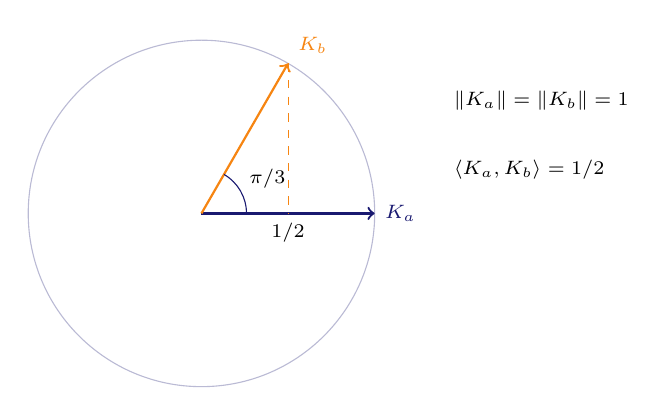
\begin{tikzpicture}[scale=2.2,every node/.style={font=\scriptsize}]
\draw[MidnightBlue!30] (0,0) circle (1);
\draw[->,thick,MidnightBlue] (0,0)--(1,0) node[right] {$K_a$};
\draw[->,thick,BurntOrange] (0,0)--(0.5,0.8660254) node[above right] {$K_b$};
\draw[MidnightBlue] (0.26,0) arc (0:60:0.26);
\node at (0.38,0.2) {$\pi/3$};
\draw[BurntOrange,dashed] (0.5,0.8660254)--(0.5,0);
\node[below] at (0.5,0) {$1/2$};
\node[anchor=west] at (1.4,0.65) {$\|K_a\|=\|K_b\|=1$};
\node[anchor=west] at (1.4,0.25) {$\langle K_a,K_b\rangle=1/2$};
\end{tikzpicture}
